% Control stack with the planned supraspinal additions (Chapter 7,
% sec:fw_senses).  Compile: pdflatex -output-directory=.. sensorium_hierarchy.tex
% Every inter-tier arrow runs in its own lane with its label on the side
% away from neighboring lanes; the future closure is drawn from the body box
% to the vestibular and ocular box at the far right.
\documentclass[border=6pt]{standalone}
\usepackage[T1]{fontenc}
\usepackage{mathpazo}
\usepackage{tikz}
\usetikzlibrary{arrows.meta, positioning, calc}
\begin{document}
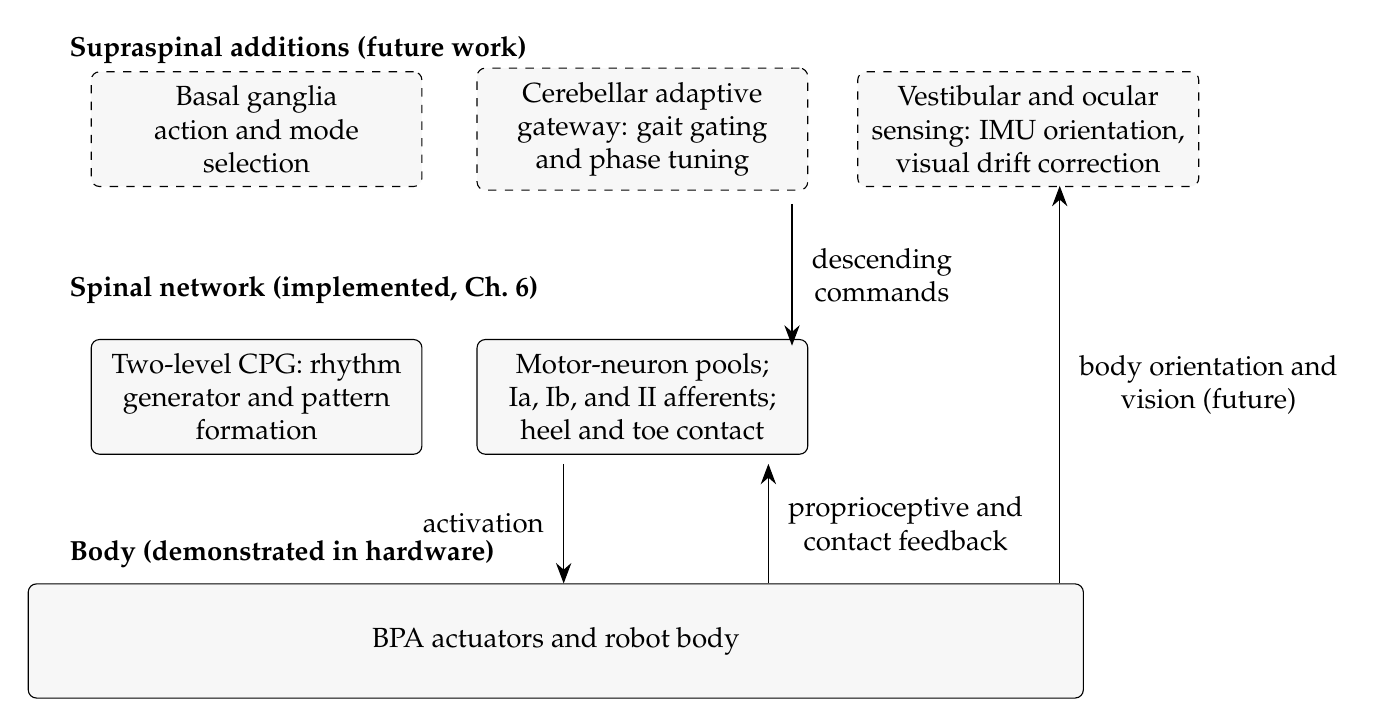
\begin{tikzpicture}[
  font=\normalsize,
  box/.style={draw, rounded corners=3pt, align=center, inner sep=5pt,
              minimum width=4.2cm, minimum height=1.45cm, fill=black!3},
  future/.style={box, dashed},
  arrow/.style={-{Stealth[length=2.6mm]}, thin, rounded corners=6pt},
  lab/.style={align=center, inner sep=3pt},
  tier/.style={font=\normalsize\bfseries, anchor=west},
]

% Tier captions, each above its tier and clear of the arrow lanes
\node[tier] at (0,2.05) {Supraspinal additions (future work)};
\node[tier] at (0,-1.00) {Spinal network (implemented, Ch.~6)};
\node[tier] at (0,-4.35) {Body (demonstrated in hardware)};

% Supraspinal tier: basal ganglia, cerebellar gateway, vestibular and ocular
\node[future] (bg)   at (2.50,1.05) {Basal ganglia\\action and mode\\selection};
\node[future] (cb)   at (7.40,1.05) {Cerebellar adaptive\\gateway: gait gating\\and phase tuning};
\node[future] (vest) at (12.30,1.05){Vestibular and ocular\\sensing: IMU orientation,\\visual drift correction};
% Spinal tier
\node[box] (cpg) at (2.50,-2.35) {Two-level CPG: rhythm\\generator and pattern\\formation};
\node[box] (mn)  at (7.40,-2.35) {Motor-neuron pools;\\Ia, Ib, and II afferents;\\heel and toe contact};
% Body tier
\node[box, minimum width=13.4cm] (body) at (6.30,-5.45) {BPA actuators and robot body};

% Descending commands, own lane under the gateway box
\draw[arrow] (9.30,0.10) -- node[lab, right=4pt] {descending\\commands} (9.30,-1.70);
% Activation down, label on the left
\draw[arrow] (6.40,-3.20) -- node[lab, left=4pt] {activation} (6.40,-4.72);
% Proprioceptive and contact feedback up, label on the right
\draw[arrow] (9.00,-4.72) -- node[lab, right=4pt] {proprioceptive and\\contact feedback} (9.00,-3.20);
% Future closure: body orientation and vision, far-right lane into the
% vestibular and ocular box
\draw[arrow] (12.70,-4.72) -- node[lab, right=4pt] {body orientation and\\vision (future)} (12.70,0.33);

\end{tikzpicture}
\end{document}
